\chapter{PENGEMBANGAN MODEL DETEKSI PERILAKU PELANGGARAN PENYEWA}
\label{chap:model}

Bab ini menguraikan tahapan pengembangan model pembelajaran mesin secara komprehensif dengan menerapkan siklus \textit{data science} lanjutan pasca perumusan masalah yang telah dibahas pada Bab 3. Cakupan alur proses ini dimulai dari pengumpulan dan persiapan data, penanganan ketidakseimbangan kelas, pemilihan serta pelatihan beberapa algoritma klasifikasi, evaluasi performa model, hingga pemilihan dan ekspor model terbaik. Setiap tahapan proses secara rinci beserta potongan kode program dan hasil eksekusi lengkapnya dapat dilihat pada Lampiran~\ref{lamp:A}. Model terbaik yang dihasilkan dari rangkaian proses tersebut selanjutnya dipersiapkan untuk diintegrasikan secara langsung (\textit{embedded}) ke dalam sistem \textit{data capture} guna mendukung mekanisme deteksi dini potensi perilaku pelanggaran penyewa di lingkungan hunian.



% Sub-bab 4.1 Pengumpulan Data
\section{Pengumpulan Data}

Sumber data utama dalam penelitian ini mengacu pada skema basis data \texttt{rentals} dari sistem pencatatan penyewaan unit di lingkungan Rusunami The Jarrdin Cihampelas (RTJC). Secara operasional, data ini dikumpulkan secara langsung melalui aplikasi {Data Capture} yang dapat diakses melalui tautan \texttt{visitor.thejarrdin.com}. Melalui aplikasi tersebut, sistem mencatat riwayat kedatangan penyewa beserta rekam jejak pelanggarannya secara terpusat. Data operasional ini kemudian diekstrak ke dalam beberapa berkas (\textit{dataset}), yakni \texttt{rentals.csv}, \texttt{rental\_logs.csv}, \texttt{units.csv}, dan \texttt{violations.csv}. Nama kolom pada seluruh berkas tersebut diseragamkan menggunakan format huruf kecil (\textit{lowercasing}) untuk mempermudah tahapan pemrosesan.

Pada tahapan awal, penelitian ini menggunakan dataset sintetis karena sistem belum memiliki data historis riil untuk pelatihan \textit{machine learning}. Karakteristik, distribusi, dan anomali data disimulasikan menggunakan \textit{seeder} (berupa \texttt{index.js} dan skema injeksi \texttt{seeder.sql}) serta pustaka \texttt{Faker} untuk menjamin variasi data identitas yang disesuaikan dengan kondisi faktual berdasarkan hasil wawancara narasumber. 

Namun pada tahap revisi dan operasional saat ini, penelitian telah sepenuhnya menggunakan dataset riil yang diekstrak langsung dari kegiatan operasional harian sistem penyewaan RTJC. Mengingat sistem telah berjalan dan berhasil menghimpun data historis riil dalam jumlah yang cukup untuk pelatihan \textit{machine learning}, dataset ini secara langsung merepresentasikan karakteristik, distribusi, dan kejadian anomali yang faktual terjadi di lapangan. Proses perolehan data tidak lagi bergantung pada pustaka \texttt{Faker} atau \textit{seeder}, melainkan murni bersumber dari rekaman aktivitas nyata para penyewa.

Dalam pengumpulan data riil ini jika ditemukan indikasi pelanggaran, maka petugas pengelola secara langsung dengan melakukan input ``komentar''. Penyewa yang menyalahgunakan unit untuk tujuan ``transit'' akan tercatat di dalam sistem dengan pola yang khas, seperti durasi sewa yang sangat pendek serta waktu \textit{check-in} pada jam-jam yang tidak lazim.

Informasi (atribut) di dalam kumpulan data tersebut kemudian disaring untuk mengambil kolom yang paling relevan. Data yang merangkum pola perilaku penyewa ini disatukan ke dalam satu struktur tabel dengan rincian sebagai berikut.
\begin{itemize}
    \item \textbf{Identitas penyewa:} mencakup atribut NIK (Nomor Induk Kependudukan) dan nama untuk memastikan serta melacak profil penyewa.
    \item \textbf{Profil demografis:}
    \begin{itemize}
        \item \texttt{status\_pasutri}: menandakan status pernikahan (`Menikah' atau `Belum Menikah'). Informasi ini krusial untuk mendeteksi potensi pelanggaran aturan terkait norma sosial atau asusila.
        \item \texttt{status\_kewarganegaraan}: membedakan asal negara penyewa, yakni `WNI' atau `WNA'.
    \end{itemize}
    \item \textbf{Detail transaksi sewa:}
    \begin{itemize}
        \item \texttt{jenis\_sewa}: kategori masa sewa (`Harian', `Mingguan', atau `Bulanan').
        \item \texttt{metode\_pembayaran}: mekanisme pembayaran yang dipilih oleh penyewa (Tunai, Kartu Debit, dan sebagainya). 
    \end{itemize}
    \item \textbf{Data temporal (waktu):}
    \begin{itemize}
        \item \texttt{tanggal\_checkin} dan \texttt{waktu\_checkin}: informasi penanda hari dan jam kedatangan penyewa.
        \item \texttt{tanggal\_checkout} dan \texttt{waktu\_checkout}: informasi penanda hari dan jam batas akhir penyewaan.
        \item \texttt{lama\_menginap}: total durasi atau lamanya penyewa menetap di dalam unit.
    \end{itemize}
\end{itemize}

Seluruh kumpulan informasi ini memegang peran esensial sebagai fondasi awal bagi model \textit{machine learning} untuk mengidentifikasi kebiasaan penyewa. Melalui rekaman pola-pola tersebut, sistem mampu memprediksi profil penyewa yang memiliki kecenderungan untuk melakukan pelanggaran tata tertib di kemudian hari.

% Sub-bab 4.2 Penyiapan Data
\section{Penyiapan Data dan Pelabelan}

Tahap penyiapan data berfokus pada pembersihan data awal dan pemberian label (\textit{labeling}) untuk pengelompokan data. Label sangat penting untuk melatih algoritma pembelajaran (\textit{supervised learning}) seperti yang dibahas pada Subbab~\ref{sec:machine_learning}. Dalam sistem ini, data penyewa yang telah dikumpulkan akan diseragamkan terlebih dahulu menjadi huruf kecil (lowercasing) dan dihilangkan spasi berlebihnya (stripping). Setelah itu, data akan diberikan nilai berupa angka 0 atau 1 (skor biner). Nilai ini ditentukan secara otomatis dari ada atau tidaknya catatan pelanggaran pada kolom komentar, dengan aturan matematis sebagai berikut.

\[
Label(x) =
\begin{cases}
0, & \text{jika } komentar \in \{ \text{kosong, ``nan'', ``na'', ``null'', ``-'', ``0'', ``tidak ada'', ``none'', spasi} \} \\
1, & \text{lainnya (terdapat catatan pelanggaran)}
\end{cases}
\]

Pendekatan ini memisahkan penyewa ke dalam dua kelompok utama:
\begin{itemize}
    \item \textbf{Kelas Normal (0):} penyewa yang mematuhi aturan dan riwayat catatannya bersih dari pelanggaran.
    \item \textbf{Kelas Tidak Normal (1):} penyewa yang terindikasi melanggar aturan dan menimbulkan kerugian bagi pihak pengelola.
\end{itemize}

Melalui proses penyiapan data dan pelabelan ini, model algoritma dapat menggunakan angka 0 dan 1 tersebut sebagai patokan dasar. Tujuannya adalah agar sistem mampu mengenali pola kebiasaan yang tidak wajar (\textit{anomali}) berdasarkan informasi transaksi penyewa lainnya.

% Sub-bab 4.3 EDA
\section{\textit{Exploratory Data Analysis} (EDA)}

Tahapan \textit{Exploratory Data Analysis} (EDA) bertujuan untuk mengenali karakteristik data dan mengidentifikasi pola hubungan di dalamnya sebelum diproses menggunakan algoritma pembelajaran mesin. Mengingat penelitian ini mengalami transisi dari penggunaan data sintetis (\textit{dummy}) menuju data operasional riil, tahapan EDA juga berperan penting dalam memvalidasi asumsi penelitian. Kemiripan maupun perbedaan pola yang ditemukan antara data sintetis dan data riil memberikan landasan empiris yang kuat, mengingat data sintetis tersebut sejak awal telah dirancang untuk merepresentasikan estimasi kondisi faktual penyewa di lapangan.

\subsection{Distribusi Kelas Target}
Pada tahap awal, distribusi kelas target disimulasikan menggunakan data sintetis dengan perbandingan penyewa Normal (Aman) berlabel 0 sebanyak 9.243 data, berbanding penyewa Tidak Normal (Melanggar) berlabel 1 sebanyak 746 data. Setelah sistem beroperasi, ekstraksi pada data riil memvalidasi proporsi ketimpangan tersebut, di mana diperoleh 453 data penyewa Normal dan 88 data penyewa Melanggar. Grafik perbandingan pada Gambar~\ref{fig:dist_kelas} memperlihatkan konsistensi ketimpangan jumlah data yang sangat besar (\textit{class imbalance}) pada kedua skenario. Kondisi ini dapat menyebabkan algoritma bias dan cenderung hanya memprediksi kelas mayoritas (penyewa normal). Oleh karena itu, ketimpangan ini wajib ditangani menggunakan sistem penalti pembobotan (\textit{cost-sensitive learning}) pada tahapan pelatihan model.

\begin{figure}[H]
    \centering
    \begin{subfigure}[b]{0.45\textwidth}
        \centering
        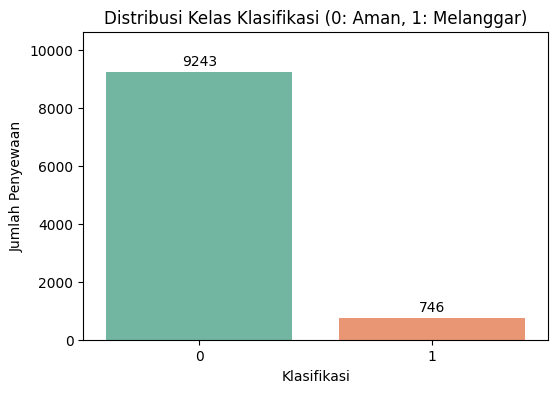
\includegraphics[width=\textwidth]{Gambar/Distribusi_Kelas_Dummy.png}
        \caption{Data Sintetis (\textit{Dummy})}
        \label{fig:dist_kelas_dummy}
    \end{subfigure}
    \hfill
    \begin{subfigure}[b]{0.45\textwidth}
        \centering
        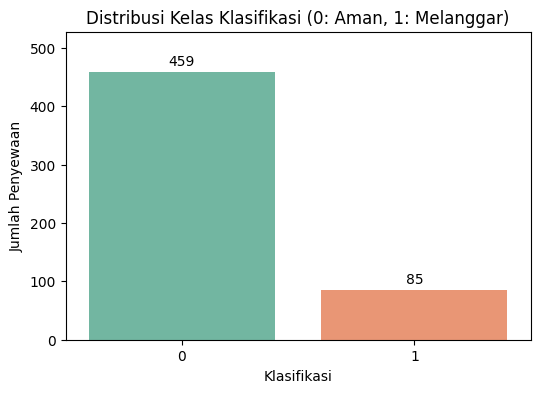
\includegraphics[width=\textwidth]{Gambar/Distribusi_Kelas_Riil.png}
        \caption{Data Riil}
        \label{fig:dist_kelas_riil}
    \end{subfigure}
    \caption{Perbandingan Distribusi Kelas Klasifikasi (0: Aman, 1: Melanggar)}
    \label{fig:dist_kelas}
\end{figure}

\subsection{Korelasi Antar Fitur Temporal (\textit{Heatmap})}
Analisis korelasi diterapkan pada fitur numerik untuk mengukur atribut yang paling berpengaruh terhadap label klasifikasi. Pada data sintetis, korelasi sengaja dibentuk berdasarkan hipotesis awal mengenai perilaku penyewa, di mana jam kedatangan (\textit{check-in}) dan lama menginap diasumsikan memiliki korelasi negatif terhadap label, masing-masing sebesar -0,24 dan -0,22. Hipotesis simulasi ini terbukti sangat relevan pada fitur lama menginap. \textit{Heatmap} data riil secara empiris justru mengonfirmasi keberadaan korelasi negatif yang melesat menjadi jauh lebih kuat, yakni mencapai -0,52 terhadap label pelanggaran. Peningkatan angka korelasi ini menegaskan bahwa semakin singkat durasi menginap seorang penyewa, semakin tinggi pula kemungkinan penyewa tersebut melakukan pelanggaran. 

Di sisi lain, terjadi perbedaan temuan pada variabel jam \textit{check-in}. Berbeda dengan asumsi sintetis yang memiliki korelasi -0,24, variabel jam kedatangan pada operasional riil sama sekali tidak menunjukkan korelasi (0,00) terhadap label. Penurunan drastis ini mengindikasikan adanya pergeseran pola di lapangan yang berbeda dari estimasi awal, di mana penyewa yang melanggar pada kondisi nyata tidak lagi memiliki kecenderungan kuat untuk datang pada jam-jam spesifik (seperti tengah malam), melainkan datang pada jam operasional yang wajar. Selain itu, pada data riil fitur seperti jenis sewa dan kewarganegaraan tidak memunculkan nilai korelasi karena seluruh transaksi riil murni berasal dari penyewa harian berkewarganegaraan WNI (tidak ada variansi data).

\begin{figure}[H]
    \centering
    \begin{subfigure}[b]{0.45\textwidth}
        \centering
        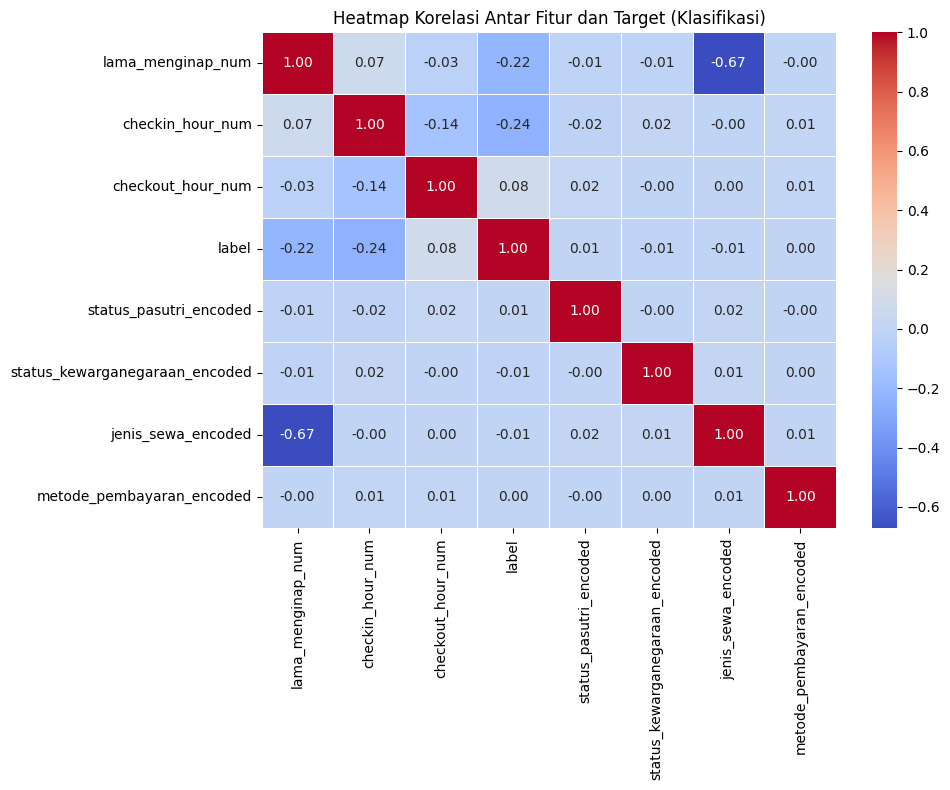
\includegraphics[width=\textwidth]{Gambar/Heatmap_Korelasi_Dummy.png}
        \caption{Data Sintetis (\textit{Dummy})}
        \label{fig:heatmap_korelasi_dummy}
    \end{subfigure}
    \hfill
    \begin{subfigure}[b]{0.45\textwidth}
        \centering
        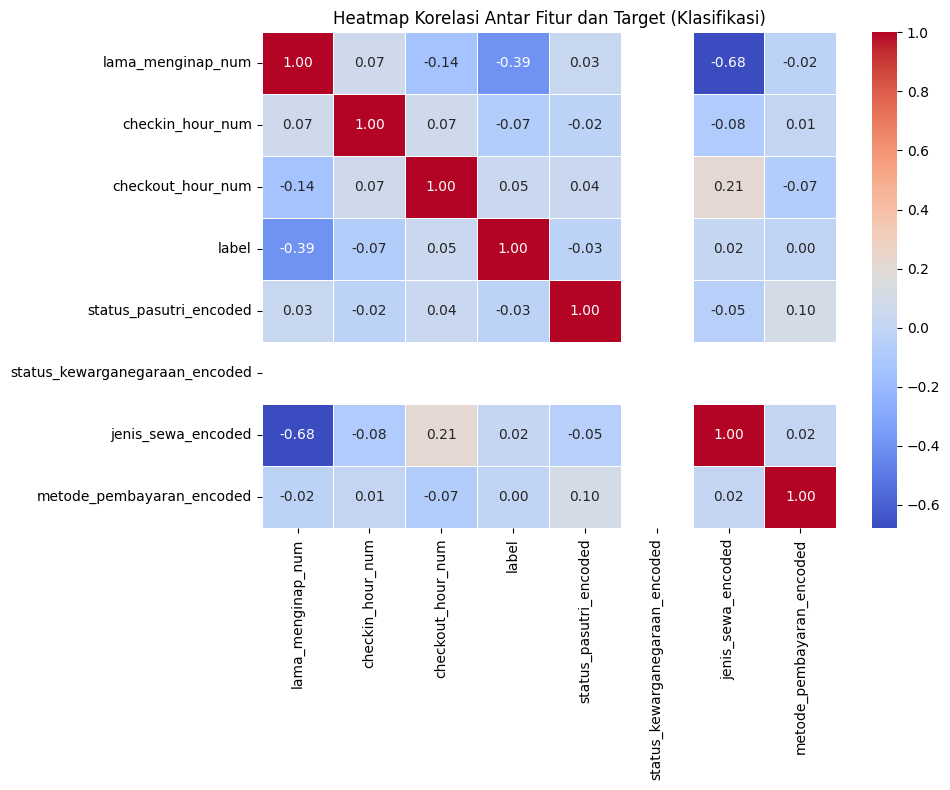
\includegraphics[width=\textwidth]{Gambar/Heatmap_Korelasi_Riil.png}
        \caption{Data Riil}
        \label{fig:heatmap_korelasi_riil}
    \end{subfigure}
    \caption{Heatmap Korelasi Antar Fitur dan Target}
    \label{fig:heatmap_korelasi}
\end{figure}

\subsection{Visualisasi Pola Penyewaan}
Tahap eksplorasi selanjutnya adalah membandingkan pola transaksi penyewa antara skenario simulasi dan kejadian nyata di lapangan.
\begin{enumerate}
    \item \textbf{Pola Jam \textit{Check-in}}\\ 
    Terdapat perbedaan temuan yang signifikan antara skenario simulasi dan operasional nyata. Pada data sintetis, asumsi awal menduga tingginya aktivitas kedatangan penyewa tidak normal terjadi secara spesifik pada jam-jam sepi (antara pukul 00:00 hingga 05:00 WIB). Namun, grafik pada Gambar~\ref{fig:pola_waktu} mengonfirmasi bahwa pada operasional riil di lapangan, seluruh aktivitas kedatangan penyewa (baik aman maupun melanggar) murni berpusat pada siang hingga malam hari, yakni di rentang pukul 13:00 hingga 20:00 WIB. Fakta ini menjelaskan bahwa pada kondisi nyata, pelanggaran tidak selalu terikat pada jam kedatangan yang tidak lazim.
    
    \begin{figure}[H]
        \centering
        \begin{subfigure}[b]{0.45\textwidth}
            \centering
            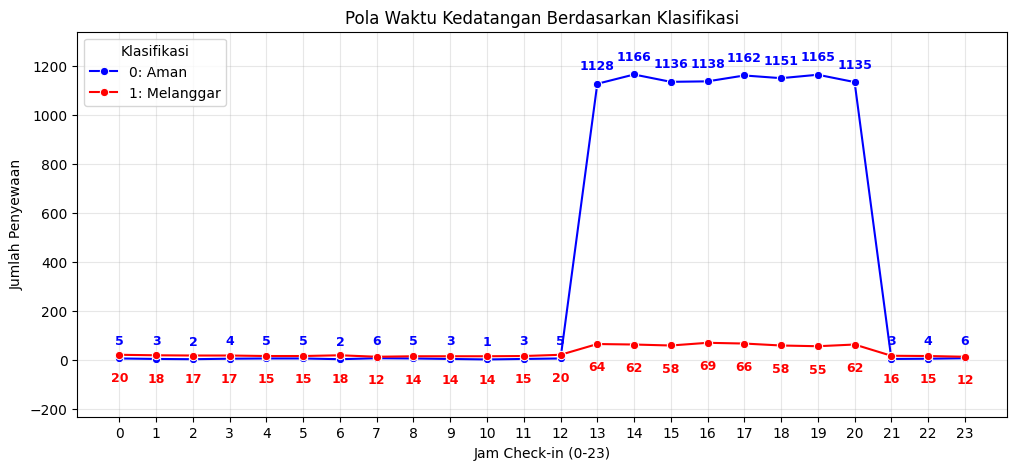
\includegraphics[width=\textwidth]{Gambar/Pola_Waktu_Kedatangan_Dummy.png}
            \caption{Data Sintetis (\textit{Dummy})}
            \label{fig:pola_waktu_dummy}
        \end{subfigure}
        \hfill
        \begin{subfigure}[b]{0.45\textwidth}
            \centering
            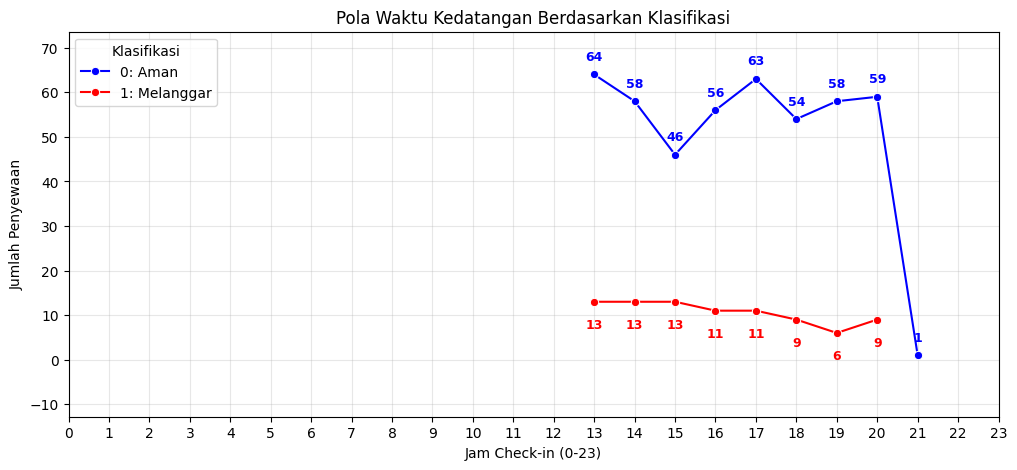
\includegraphics[width=\textwidth]{Gambar/Pola_Waktu_Kedatangan_Riil.png}
            \caption{Data Riil}
            \label{fig:pola_waktu_riil}
        \end{subfigure}
        \caption{Pola Waktu Kedatangan Berdasarkan Klasifikasi}
        \label{fig:pola_waktu}
    \end{figure}

    \item \textbf{Tren Lama Menginap}\\ 
    Sejalan dengan nilai korelasi kuat pada matriks sebelumnya, Gambar~\ref{fig:tren_menginap} membuktikan bahwa asumsi perancangan data sintetis sejalan dengan fakta di lapangan. Baik pada lingkungan simulasi maupun lingkungan nyata, kasus pelanggaran secara mutlak didominasi oleh penyewa dengan durasi inap yang sangat pendek. Pada data riil, 100\% kasus pelanggaran (88 kasus) terkonsentrasi hanya pada penyewa dengan lama inap 1 hari. Sebaliknya, penyewa dengan durasi inap jangka menengah hingga panjang terbukti memiliki profil yang sepenuhnya aman dari catatan pelanggaran.
    
    \begin{figure}[H]
        \centering
        \begin{subfigure}[b]{0.45\textwidth}
            \centering
            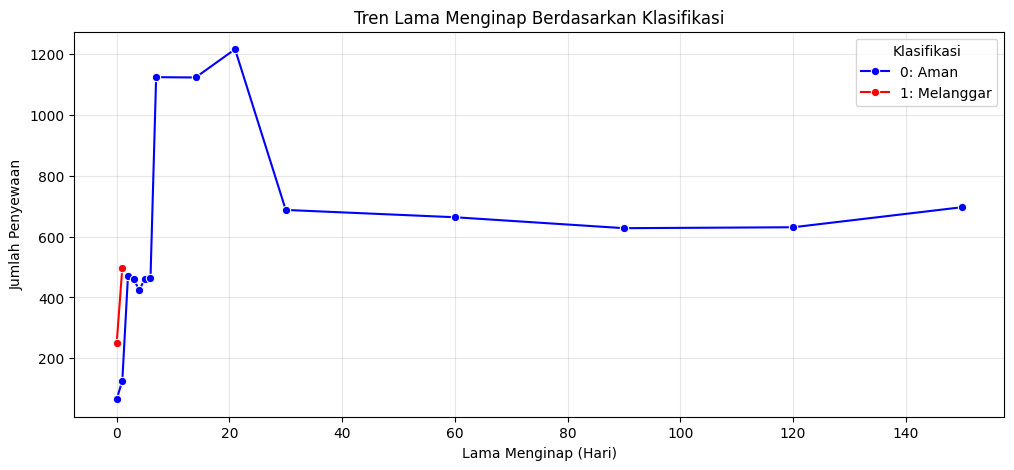
\includegraphics[width=\textwidth]{Gambar/Tren_Lama_Menginap_Dummy.png}
            \caption{Data Sintetis (\textit{Dummy})}
            \label{fig:tren_menginap_dummy}
        \end{subfigure}
        \hfill
        \begin{subfigure}[b]{0.45\textwidth}
            \centering
            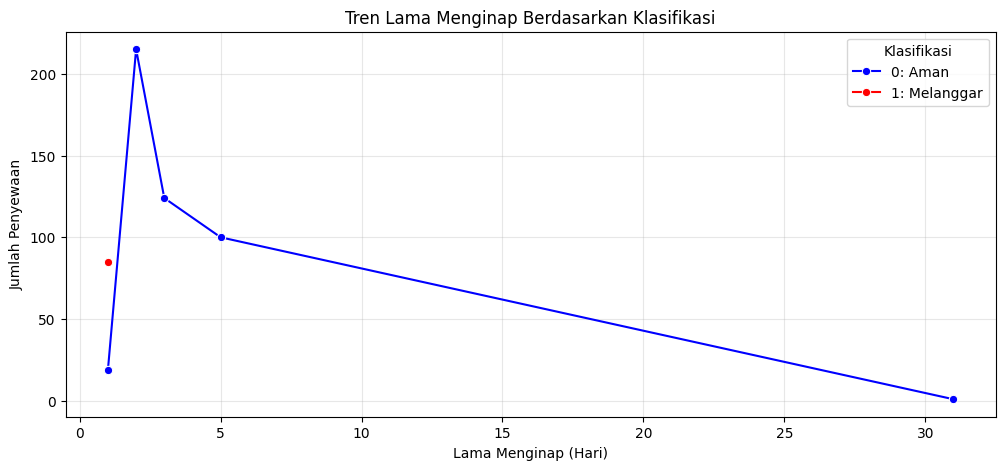
\includegraphics[width=\textwidth]{Gambar/Tren_Lama_Menginap_Riil.png}
            \caption{Data Riil}
            \label{fig:tren_menginap_riil}
        \end{subfigure}
        \caption{Tren Lama Menginap Berdasarkan Klasifikasi}
        \label{fig:tren_menginap}
    \end{figure}

    \item \textbf{Perbandingan Variabel Kategori}\\ 
    Berdasarkan Gambar~\ref{fig:jenis_sewa}, seluruh operasional nyata, termasuk 88 kasus pelanggaran murni didominasi oleh jenis sewa ``Harian''. Berbeda dengan data sintetis yang masih mensimulasikan penyewaan ``Mingguan'' dan ``Bulanan''. Perbedaan pola data operasional riil membuktikan bahwa asumsi simulasi sebelumnya mengenai tingginya risiko anomali yang hanya berpusat pada penyewa transit harian jangka pendek adalah benar.
    
    \begin{figure}[H]
        \centering
        \begin{subfigure}[b]{0.45\textwidth}
            \centering
            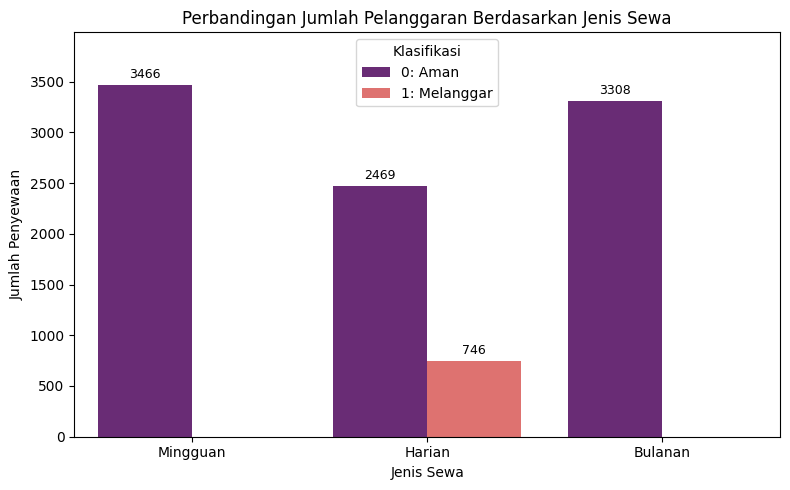
\includegraphics[width=\textwidth]{Gambar/Perbandingan_Jenis_Sewa_Dummy.png}
            \caption{Data Sintetis (\textit{Dummy})}
            \label{fig:jenis_sewa_dummy}
        \end{subfigure}
        \hfill
        \begin{subfigure}[b]{0.45\textwidth}
            \centering
            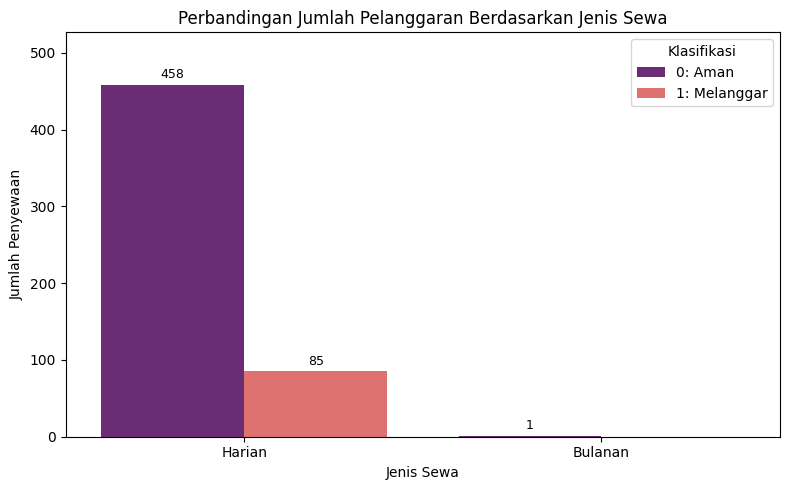
\includegraphics[width=\textwidth]{Gambar/Perbandingan_Jenis_Sewa_Riil.png}
            \caption{Data Riil}
            \label{fig:jenis_sewa_riil}
        \end{subfigure}
        \caption{Perbandingan Jumlah Pelanggaran Berdasarkan Jenis Sewa}
        \label{fig:jenis_sewa}
    \end{figure}
    
    Pada atribut demografis status pernikahan (Gambar~\ref{fig:status_pasutri}) menunjukkan pola yang sama dengan data sintetis, di mana pelanggaran pada data riil tersebar secara ekuivalen (masing-masing tepat 44 kasus) pada kelompok Menikah dan Belum Menikah. Sementara itu, pada status kewarganegaraan (Gambar~\ref{fig:status_kewarganegaraan}), keseluruhan data operasional riil murni diisi oleh WNI, yang mana meniadakan distribusi risiko pada WNA seperti yang sebelumnya disimulasikan pada data sintetis.
    
    \begin{figure}[H]
        \centering
        \begin{subfigure}[b]{0.45\textwidth}
            \centering
            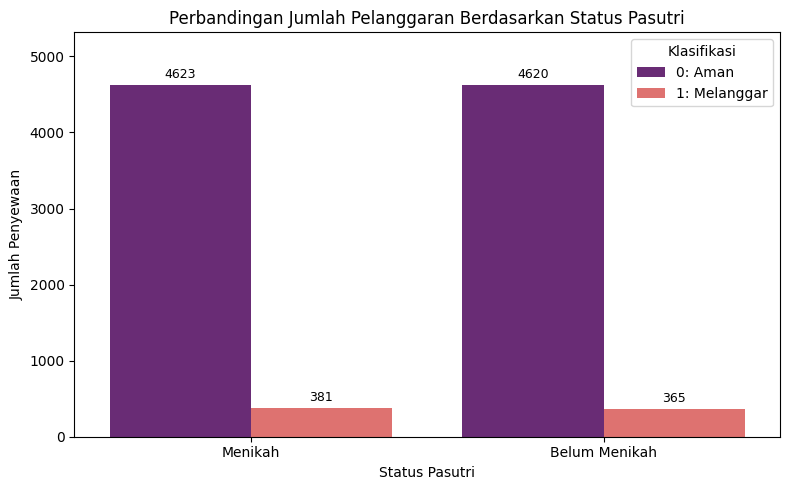
\includegraphics[width=\textwidth]{Gambar/Perbandingan_Status_Pasutri_Dummy.png}
            \caption{Data Sintetis (\textit{Dummy})}
            \label{fig:status_pasutri_dummy}
        \end{subfigure}
        \hfill
        \begin{subfigure}[b]{0.45\textwidth}
            \centering
            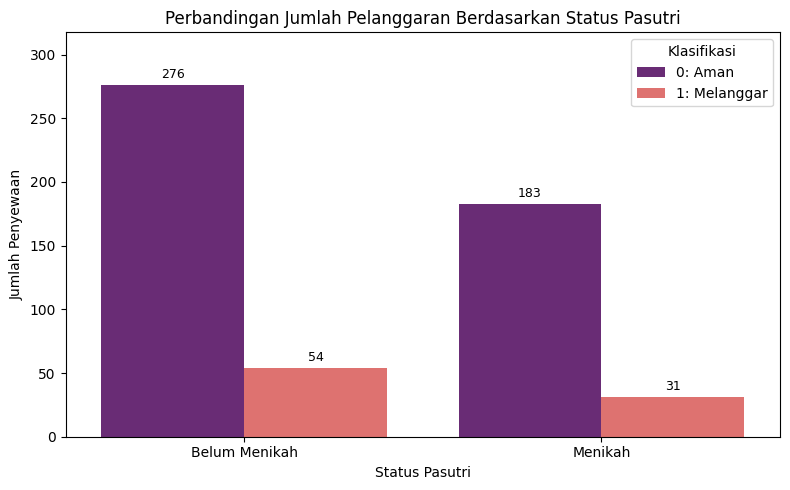
\includegraphics[width=\textwidth]{Gambar/Perbandingan_Status_Pasutri_Riil.png}
            \caption{Data Riil}
            \label{fig:status_pasutri_riil}
        \end{subfigure}
        \caption{Perbandingan Jumlah Pelanggaran Berdasarkan Status Pasutri}
        \label{fig:status_pasutri}
    \end{figure}

    \begin{figure}[H]
        \centering
        \begin{subfigure}[b]{0.45\textwidth}
            \centering
            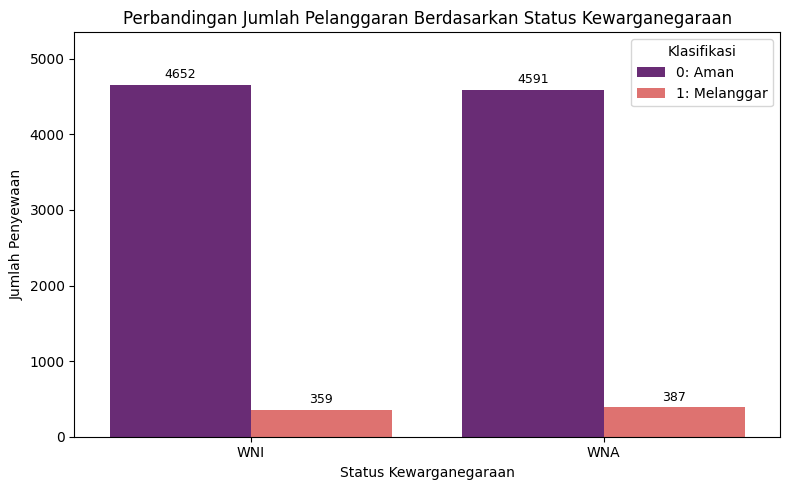
\includegraphics[width=\textwidth]{Gambar/Perbandingan_Status_Kewarganegaraan_Dummy.png}
            \caption{Data Sintetis (\textit{Dummy})}
            \label{fig:status_kewarganegaraan_dummy}
        \end{subfigure}
        \hfill
        \begin{subfigure}[b]{0.45\textwidth}
            \centering
            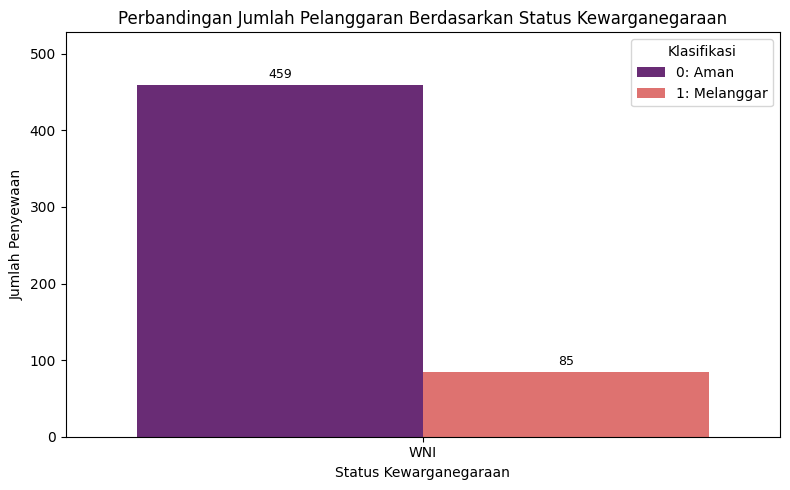
\includegraphics[width=\textwidth]{Gambar/Perbandingan_Status_Kewarganegaraan_Riil.png}
            \caption{Data Riil}
            \label{fig:status_kewarganegaraan_riil}
        \end{subfigure}
        \caption{Perbandingan Jumlah Pelanggaran Berdasarkan Status Kewarganegaraan}
        \label{fig:status_kewarganegaraan}
    \end{figure}

    Terakhir, visualisasi metode pembayaran terlihat pada Gambar~\ref{fig:metode_pembayaran}. Berbeda dengan data sintetis yang mengasumsikan distribusi merata, data riil memperlihatkan bahwa pelanggaran paling banyak tercatat pada transaksi digital seperti \textit{Others} (36 kasus) dan QRIS (27 kasus), disusul oleh transaksi Tunai/\textit{Cash} (20 kasus). Penggunaan kartu kredit dan debit justru terbukti memiliki risiko pelanggaran yang sangat minim di lapangan. Pada rancangan data sintetis, opsi \textit{Others} diasumsikan memiliki variansi yang tinggi dan tersebar secara hampir merata pada berbagai macam platform digital kekinian (seperti Paylater, Ovo, Shopeepay, Gopay, hingga Crypto) dengan rentang 275 hingga 297 transaksi per metode. Namun, fakta pada operasional data riil menunjukkan bahwa kategori \textit{Others} justru secara mutlak didominasi oleh metode konvensional berupa ``Transfer'' (227 transaksi), sementara sisanya menggunakan metode ``Aplikasi'' yang hanya tercatat sebanyak 1 transaksi. Temuan ini membuktikan bahwa pada praktiknya di lapangan, opsi pembayaran alternatif penyewa nyatanya tidak bervariasi dan hanya terpusat pada metode transfer bank.

    \begin{figure}[H]
        \centering
        \begin{subfigure}[b]{0.45\textwidth}
            \centering
            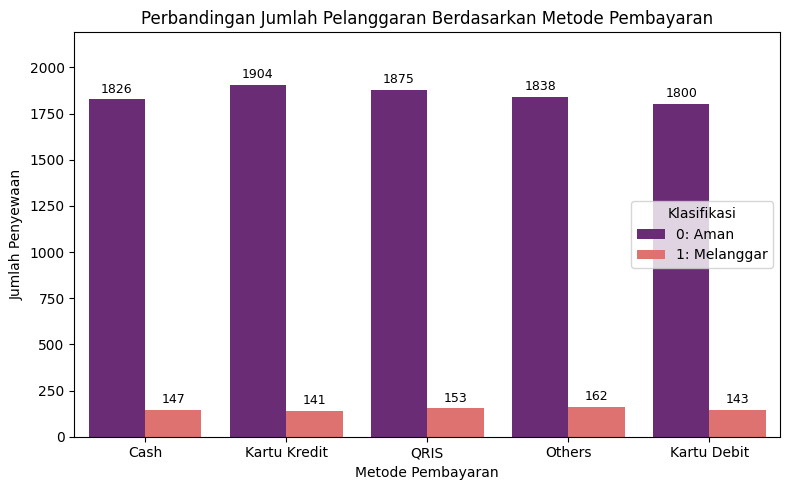
\includegraphics[width=\textwidth]{Gambar/Perbandingan_Metode_Pembayaran_Dummy.png}
            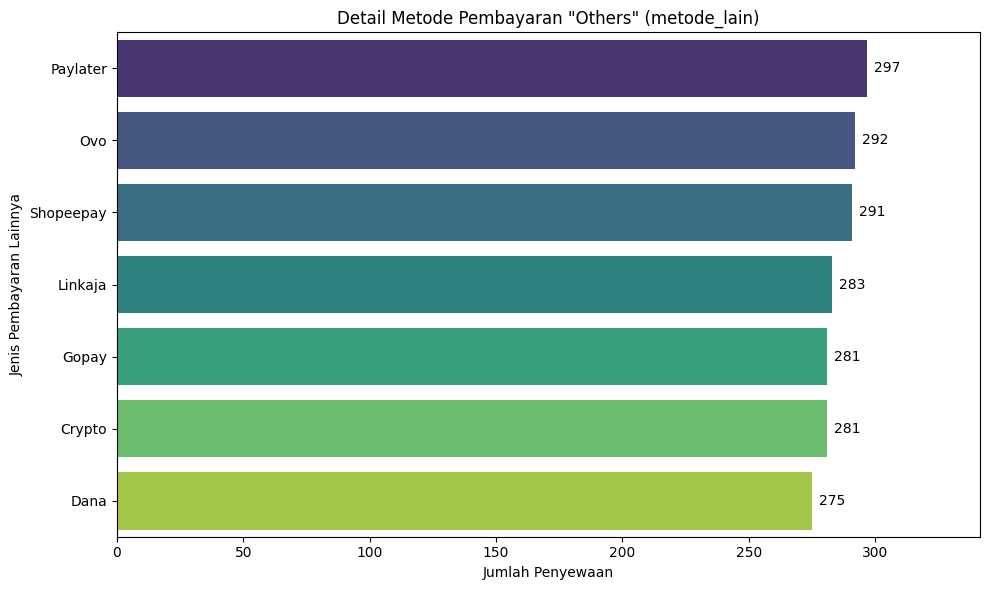
\includegraphics[width=\textwidth]{Gambar/Detail_Others_Dummy.png}
            \caption{Data Sintetis (\textit{Dummy})}
            \label{fig:metode_pembayaran_dummy}
        \end{subfigure}
        \hfill
        \begin{subfigure}[b]{0.45\textwidth}
            \centering
            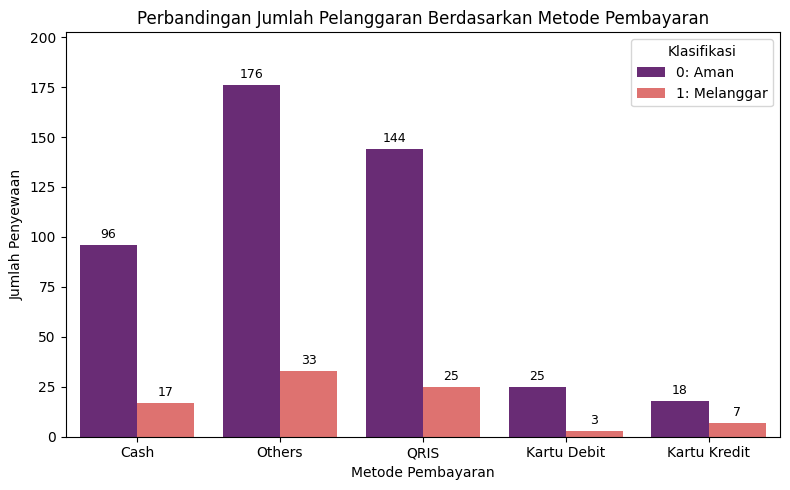
\includegraphics[width=\textwidth]{Gambar/Perbandingan_Metode_Pembayaran_Riil.png}
            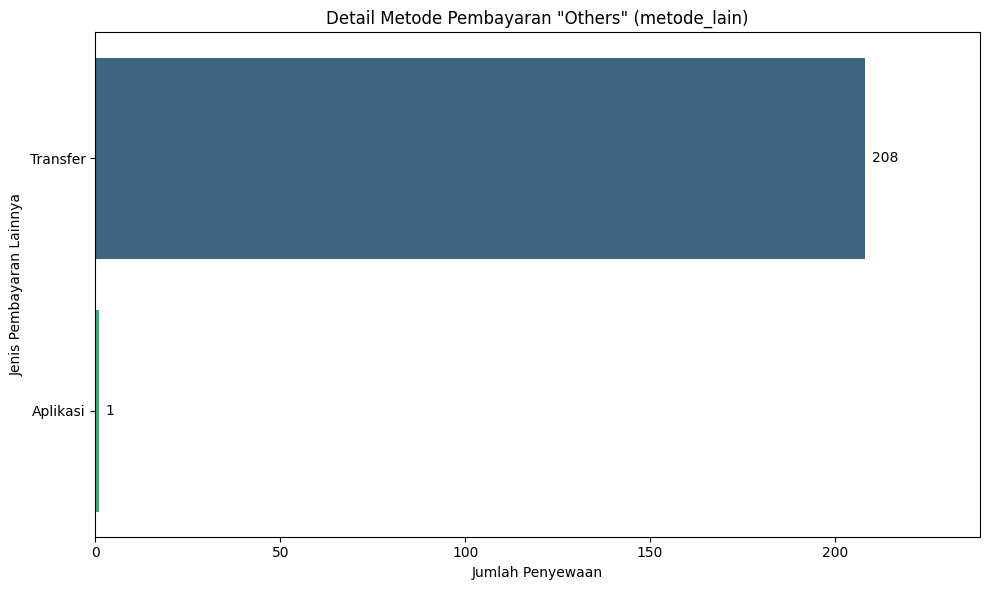
\includegraphics[width=\textwidth]{Gambar/Detail_Others_Riil.png}
            \caption{Data Riil}
            \label{fig:metode_pembayaran_riil}
        \end{subfigure}
        \caption{Perbandingan Jumlah Pelanggaran Berdasarkan Metode Pembayaran}
        \label{fig:metode_pembayaran}
    \end{figure}
\end{enumerate}

% Sub-bab 4.4 Feature Engineering
\section{\textit{Feature Engineering}}

Tahap \textit{feature engineering} bertujuan untuk mengekstraksi dan merangkai parameter kunci agar datanya dapat diproses secara optimal oleh algoritma. Rekayasa fitur ini diterapkan pada variabel waktu (temporal) maupun teks kategori (kategorikal) yang belum terstruktur.
\begin{itemize}
    \item \textbf{Ekstraksi Waktu Kedatangan dan Keberangkatan}\\ Format penulisan pada kolom \texttt{waktu\_checkin} dan \texttt{waktu\_checkout} diuraikan (\textit{parsing}) menggunakan pustaka operasional waktu khusus (\texttt{pd.to\_datetime}) guna mengambil angka jam numeriknya saja. Hasil ekstraksi ini disimpan ke dalam fitur baru bernama \texttt{checkin\_hour} dan \texttt{checkout\_hour} dengan rentang nilai bulat 0 hingga 23.
    \item \textbf{Penanganan Nilai Kosong (\textit{Missing Values}) Numerik}\\ Kolom yang memuat angka durasi, seperti \texttt{lama\_menginap}, sering kali memiliki baris yang kosong atau tidak valid (\textit{null/NaN}). Data tersebut diubah ke dalam tipe numerik menjadi angka $0$.
    \item \textbf{Penanganan (\textit{Encoding}) Data Kategorikal}\\ Beberapa kolom memiliki bentuk teks klasifikasi, seperti \texttt{jenis\_sewa}, \texttt{metode\_pembayaran}, \texttt{status\_pasutri}, dan \texttt{status\_kewarganegaraan}. Untuk menangani sel yang kosong pada kolom-kolom tersebut, nilai yang hilang diganti secara seragam dengan label teks \texttt{'Unknown'}. Selanjutnya, seluruh kategori teks tersebut dikonversi menjadi urutan angka menggunakan metode standar \textit{Label Encoding} (misalnya Harian menjadi 0, Mingguan menjadi 1, dan Bulanan menjadi 2). Konversi angka dari label ini memastikan bahwa perhitungan matematis saat pelatihan klasifikasi dapat berjalan lancar tanpa terhambat oleh masalah tipe data \textit{string}. 
\end{itemize}

% Sub-bab 4.5 Train-Test Split
\section{Pembagian Data (\textit{Train-Test Split})}

Untuk memastikan algoritma tidak sekadar menghafal sekumpulan data historis melainkan benar-benar mampu mengenali pola perilaku secara umum (\textit{generalisasi}), seluruh himpunan data operasional dipisahkan ke dalam dua bagian utama, yaitu data latih (\textit{train}) dan data uji (\textit{test}). Berdasarkan pengaturan pada sistem, pembagian dilakukan dengan rasio 80\% alokasi untuk proses pelatihan model, dan 20\% sisanya dipakai untuk pengujian akhir. Data uji sebesar 20\% ini dipisahkan sejak awal dan tidak diikutsertakan dalam tahap pelatihan, sehingga akurasi serta performa model dapat dievaluasi secara murni menggunakan \textit{unseen data} (data yang belum pernah dipelajari sebelumnya). Mengacu pada total 544 catatan riwayat penyewaan nyata di lapangan, pembagian ini menghasilkan alokasi sebanyak 435 data untuk tahap pelatihan dan 109 data sebagai parameter pengujian.

Implementasi pembagian ini tidak dilakukan secara acak, melainkan menggunakan mekanisme pembagian bertingkat (\textit{stratify}). Fungsi fundamental dari penggunaan \textit{stratify} adalah untuk menjamin agar proporsi persentase antara penyewa normal (aman) dan penyewa tidak normal (melanggar) terdistribusi dengan rasio yang identik, baik di dalam ruang data latih maupun data uji. Mengingat kondisi faktual dataset operasional sangat tidak seimbang (\textit{imbalanced data})—di mana jumlah kasus penyewa melanggar sangat minoritas—pemisahan data secara acak konvensional berisiko tinggi menyebabkan hilangnya data minoritas tersebut atau hanya condong pada salah satu partisi (misalnya, masuk seluruhnya ke data latih dan kosong di data uji). Jika anomali pemisahan itu terjadi, hasil evaluasi kemampuan deteksi algoritma akan cacat, bias, dan gagal mempresentasikan kondisi sebenarnya.

Dengan penerapan parameter \textit{stratify}, komposisi kelas target berhasil dijaga secara presisi untuk konsisten mengikuti proporsi aslinya. Bukti konkret dari keberhasilan stratifikasi ini dapat diamati secara langsung pada \textit{Classification Report} hasil pengujian model. Sebagai representasi, Tabel~\ref{tab:xgboost_report} memperlihatkan contoh cuplikan hasil pengujian dari algoritma \textit{XGBoost} versi tanpa \textit{tuning} pada data riil.

\begin{table}[H]
\centering
\caption{Cuplikan \textit{Classification Report} Model XGBoost (Tanpa \textit{Tuning}) pada Data Riil}
\label{tab:xgboost_report}
\begin{tabular}{rcccc}
\toprule
\textbf{Kelas Target} & \textbf{Precision} & \textbf{Recall} & \textbf{F1-Score} & \textbf{Support} \\
\midrule
0 (Aman) & 1.0000 & 0.9565 & 0.9778 & 92 \\
1 (Melanggar) & 0.8095 & 1.0000 & 0.8947 & 17 \\
\midrule
\textbf{Accuracy} & & & \textbf{0.9633} & \textbf{109} \\
\textbf{Macro Avg} & 0.9048 & 0.9783 & 0.9363 & 109 \\
\textbf{Weighted Avg} & 0.9703 & 0.9633 & 0.9648 & 109 \\
\bottomrule
\end{tabular}
\end{table}

Berdasarkan Tabel~\ref{tab:xgboost_report} di atas, nilai total pada kolom \textit{support} adalah 109 data uji. Data tersebut terbagi secara proporsional menjadi 92 data untuk kelas normal (label 0) dan 17 data untuk kelas melanggar (label 1). Rasio pembagian 20\% ini merepresentasikan secara presisi kondisi populasi awal yang berjumlah 544 data (459 data normal dan 85 data melanggar). Distribusi representatif inilah yang memastikan bahwa nilai evaluasi seperti \textit{precision}, \textit{recall}, dan \textit{f1-score} dapat diandalkan keabsahannya dan tidak bias terhadap kelas mayoritas.

% Sub-bab 4.6 Feature Selection
\section{Seleksi Fitur (\textit{Feature Selection})}

Sesuai dengan pembahasan pada Subbab~\ref{sec:feature_selection}, tahapan pemilihan atribut terbaik (\textit{feature selection}) diimplementasikan untuk mengurangi beban komputasi algoritma dan mengabaikan informasi yang tidak relevan (\textit{noise}). Evaluasi fitur ini dijalankan setelah himpunan data dipisahkan menjadi data latih dan data uji (\textit{train-test split}). Pendekatan ini bertujuan untuk menutup celah kebocoran informasi dari data uji ke dalam proses evaluasi fitur (\textit{data leakage}). Berikut metode yang diterapkan.
\begin{enumerate}
    \item \textbf{Uji Chi-Square (\textit{SelectKBest}):} mengevaluasi seberapa kuat dependensi antara setiap variabel kategori dengan target klasifikasi secara independen.
    \item \textbf{Uji \textit{Mutual Information}:} mengukur seberapa besar suatu fitur mampu memberikan petunjuk tambahan atau mengurangi tingkat ketidakpastian sistem dalam memprediksi kelas penyewa.
    \item \textbf{Korelasi Pearson:} mengukur kekuatan hubungan garis lurus (linear) antara fitur numerik dengan target klasifikasi, yang mana tingkat signifikansinya dinilai berdasarkan nilai absolut (\textit{absolute value}) dari koefisien korelasi.
\end{enumerate}

Untuk mengintegrasikan hasil dari tiga metrik tersebut, setiap nilai uji dinormalisasi menjadi rentang standar antara 0 hingga 1 menggunakan fungsi algoritma \texttt{MinMaxScaler}. Rata-rata dari ketiga nilai yang telah dinormalisasi kemudian dikalkulasi untuk menghasilkan satu skor akhir terpadu (\textit{Total Score}). Berdasarkan hasil eksekusi program (\textit{output}) pada tahap seleksi fitur untuk data riil, sistem melakukan pemeringkatan seluruh variabel berdasarkan skor total tertinggi, yaitu \texttt{lama\_menginap}, \texttt{checkout\_hour}, dan \texttt{checkin\_hour}. Ketiga fitur terpilih inilah yang kemudian dipakai untuk ke tahap pelatihan algoritma agar model dapat bekerja dengan tingkat komputasi yang lebih efisien serta terhindar dari bias informasi yang tidak relevan.

% Sub-bab 4.7 Melatih Model
\section{Melatih Model}

Setelah data latih (\textit{train}) disiapkan dan direduksi dimensinya menjadi empat fitur paling prediktif, tahap selanjutnya adalah melatih model \textit{machine learning}. Pada penelitian ini, pelatihan tidak menggunakan konfigurasi standar bawaan sistem (\textit{default}), melainkan menerapkan teknik optimasi parameter tingkat lanjut melalui \texttt{RandomizedSearchCV}. Teknik pencarian acak ini diinstruksikan untuk mencari dan menguji berbagai kombinasi parameter pengatur (\textit{hyperparameter tuning}) secara otomatis guna menemukan arsitektur model yang menghasilkan performa klasifikasi terbaik. Terdapat lima algoritma klasifikasi yang dilatih dan dioptimalkan secara komparatif, yakni sebagai berikut.

\begin{enumerate}
    \item \textbf{Decision Tree:} model klasifikasi dengan struktur pemecahan aturan secara berjenjang. Pencarian pengaturan optimal difokuskan pada batas maksimal tingkat kedalaman pohon aturan (\texttt{max\_depth}) dan jumlah minimal sampel observasi yang disyaratkan untuk membuat cabang aturan baru (\texttt{min\_samples\_split}). Algoritma ini juga disematkan nilai pembobotan penalti \texttt{class\_weight=\{0:1, 1:4\}} untuk memperbesar sensitivitas deteksi sistem terhadap penyewa kelas minoritas (label 1).
    \item \textbf{Random Forest:} algoritma gabungan (\textit{ensemble}) berbasis \textit{bagging} yang memproses banyak \textit{Decision Tree} secara paralel untuk meminimalisasi varians dan risiko \textit{overfitting}. Pencarian pengaturan optimal diuji pada variasi jumlah pohon yang dibangun (\texttt{n\_estimators}), tingkat kedalaman maksimal (\texttt{max\_depth}), batas minimal data pembelahan (\texttt{min\_samples\_split}), serta penempatan ujung daun (\texttt{min\_samples\_leaf}). Serupa dengan \textit{Decision Tree}, model ini menerapkan parameter pembobotan penalti dengan rasio 4:1.
    \item \textbf{K-Nearest Neighbors (KNN):} model berbasis spasial yang mengklasifikasikan data berdasarkan jarak kedekatan observasinya. Karena perhitungan metrik jarak sangat rentan terdistorsi oleh perbedaan rentang skala angka, fitur dinormalisasi terlebih dahulu menggunakan fungsi \texttt{StandardScaler} di dalam sebuah alur pemrosesan terintegrasi (\textit{pipeline}). Sistem kemudian dieksekusi untuk menguji jumlah tetangga terdekat (\texttt{n\_neighbors}) dan metode perhitungan bobot jarak (\texttt{weights}) yang paling optimal.
    \item \textbf{Support Vector Machine (SVM):} model geometris yang bertugas mencari \textit{hyperplane} (batas pemisah) terbaik antar kelas. Serupa dengan KNN, data wajib diseragamkan skalanya terlebih dahulu di dalam \textit{pipeline}, lalu dilatih menggunakan fungsi \textit{Radial Basis Function} (RBF) untuk menangkap pola sebaran data yang \textit{non-linear}. Sistem secara komputasional mencari nilai batas toleransi kesalahan (\texttt{C}) dan radius seberapa jauh pengaruh satu titik observasi tunggal terhadap batas klasifikasi (\texttt{gamma}) diiringi penerapan parameter \texttt{class\_weight} 4:1.
    \item \textbf{XGBoost:} algoritma gabungan berbasis \textit{boosting} tingkat lanjut yang membangun model secara sekuensial guna mengevaluasi dan memperbaiki rentetan kesalahan komputasi dari klasifikasi sebelumnya. Parameter ruang pencarian mencakup nilai kecepatan belajar model (\texttt{learning\_rate}), tingkat kedalaman maksimal (\texttt{max\_depth}), dan total tahapan pembentukan iterasi (\texttt{n\_estimators}). Untuk mengimbangi ketimpangan jumlah data operasional, model diatur secara eksplisit menggunakan parameter kontrol \texttt{scale\_pos\_weight=4}.
\end{enumerate}

Proses pelatihan seluruh algoritma tersebut dilakukan menggunakan himpunan data latih (\texttt{X\_train} dan \texttt{y\_train}). Selama proses pencarian parameter terbaik berlangsung, sistem menjalankan tahapan (\textit{cross-validation}) sebanyak tiga kali (\texttt{cv=3}) dan mengevaluasi kualitas setiap model menggunakan metrik \textit{F1-Macro}. Selain itu, penerapan strategi pembobotan penalti (\textit{Cost-Sensitive Learning}) pada semua algoritma memastikan bahwa proses perhitungan matematis tetap seimbang secara objektif. Langkah ini bertujuan untuk mencegah model klasifikasi menjadi bias akibat dominasi jumlah penyewa kelas normal (0) yang jauh lebih besar dibandingkan kelas melanggar (1).

% Sub-bab 4.8 Evaluasi Model
\section{Evaluasi Model}

Sesuai dengan metrik yang dipaparkan pada Subbab \ref{sec:evaluasi_model}, tahapan evaluasi dilakukan untuk mengukur kemampuan model dalam memprediksi himpunan data uji (\textit{X\_test}) yang belum pernah dipelajari sebelumnya. Kinerja setiap model dianalisis secara komprehensif melalui metrik \textit{Classification Report} guna meninjau pencapaian nilai \textit{Precision}, \textit{Recall}, serta \textit{F1-Score}. Rincian mengenai distribusi hasil prediksi klasifikasi divisualisasikan melalui \textit{Confusion Matrix}. Mengingat tujuan utama dari arsitektur sistem ini adalah untuk mendeteksi penyewa bermasalah (kelas 1), fokus evaluasi difokuskan pada metrik performa terhadap kelas minoritas agar model tidak menghasilkan peringatan keliru (\textit{false alarm}) pada sistem.

\subsection{Analisis Pengaruh Seleksi Fitur}
Sebelum membandingkan performa akhir tiap model secara spesifik, evaluasi dilakukan terhadap efektivitas jumlah fitur yang dilibatkan dalam fase pelatihan. Berdasarkan serangkaian pengujian komparatif, diperoleh kesimpulan analitis sebagai berikut.
\begin{enumerate}
    \item \textbf{Kestabilan Skenario Simulasi vs. Sensitivitas Data Riil}\\ Pada pengujian menggunakan data sintetis sebelumnya, model berbasis pohon keputusan (seperti \textit{Decision Tree}, \textit{Random Forest}, dan \textit{XGBoost}) menunjukkan performa yang sangat stabil dan tidak terpengaruh oleh reduksi dimensi fitur dengan tingkat akurasi konstan di rentang 98,30\% hingga 98,35\%. Namun, pada data riil, karakteristik tersebut memudar akibat variasi informasi yang tidak sebanyak data sintetis. Oleh karena itu, tahapan seleksi fitur—terutama penghapusan atribut statis seperti \texttt{jenis\_sewa} dan \texttt{status\_kewarganegaraan}—menjadi langkah penting guna menghindari beban \textit{noise} yang dapat merusak akurasi komputasi model.
    \item \textbf{Titik Optimal Fitur (\textit{Sweet Spot})}\\ Mengacu pada hasil keluaran seleksi fitur\ref{lamp:A}, penggunaan tiga fitur terpilih (\texttt{lama\_menginap}, \texttt{checkout\_hour}, dan \texttt{checkin\_hour}) terbukti memberikan kinerja yang optimal. Saat dikombinasikan dengan fungsi optimasi pada model misalnya KNN, susunan atribut ini berhasil membuat model berhasil mengidentifikasi 100\% kasus pelanggaran secara absolut pada himpunan data uji (dengan nilai \textit{Recall} 1,0000). Hal ini mengonfirmasi bahwa kombinasi informasi temporal tersebut berguna untuk mendeteksi anomali tanpa membebani pemrosesan atau memicu risiko \textit{overfitting}.
\end{enumerate}

\subsection{Analisis Pengaruh \textit{Hyperparameter Tuning}}
Selain penyesuaian jumlah fitur, proses pencarian parameter optimal (\textit{hyperparameter tuning}) juga memberikan pola yang bervariasi terhadap karakteristik tiap model pada data riil. Berikut adalah penjabaran hasil analisisnya.
\begin{enumerate} 
    
    % \newpage
    \item \textbf{Dampak Positif pada Model Berbasis Jarak}\\ Proses penyesuaian parameter terbukti memberikan peningkatan performa yang signifikan, khususnya pada model \textit{K-Nearest Neighbors} (KNN). Optimasi rentang jarak dan bobot tetangga mampu menaikkan nilai \textit{F1-Score} kelas minoritas dari 0,8649 (versi \textit{default}) menjadi 0,8947 (versi \textit{tuned}). Selain itu, KNN \textit{tuned} sukses mengeliminasi rasio kegagalan deteksi (\textit{False Negative}) sepenuhnya—dari 5,88\% menjadi \textit{Recall} 1,0000—dan hanya menyisakan 4 kasus (\textit{False Positive}). Sementara itu, model SVM RBF sudah mencapai performa maksimal (nilai \textit{Recall} sempurna) sejak konfigurasi \textit{default}-nya dan tidak menunjukkan perubahan performa pasca \textit{tuning}.
    \item \textbf{Dampak Stagnan pada Sebagian Model Berbasis Pohon}\\ Berbanding terbalik dengan kelompok model berbasis jarak, kinerja \textit{Decision Tree} dan \textit{XGBoost} pada data riil tidak memperlihatkan peningkatan performa. Tingkat akurasi pada \textit{Decision Tree} (96,33\%) dan \textit{XGBoost} (96,33\%) tetap stagnan dan sama persis dengan performa konfigurasi model versi \textit{default}. Model berbasis pohon ini tertahan pada angka (\textit{False Positive}) sebanyak 4 kasus. Namun, anomali positif terjadi pada \textit{Random Forest} yang berhasil memperbaiki kinerjanya dari tingkat akurasi 95,41\% (versi \textit{default}) menjadi 96,33\% setelah dilakukan \textit{tuning}.
\end{enumerate}

\subsection{Hasil Akhir Evaluasi dan Pemilihan Model Terbaik}
Kelima model klasifikasi dievaluasi kinerjanya dalam dua skenario utama, yakni pengujian menggunakan model tanpa (\textit{tuning}) dan model dengan penyesuaian parameter tingkat lanjut (\textit{hyperparameter tuning}). Pengujian final ini dieksekusi menggunakan tiga fitur terpilih, yaitu (\texttt{lama\_menginap}, \texttt{checkout\_hour}, dan \texttt{checkin\_hour}). Seluruh hasil pengujian yang mencakup nilai \textit{Precision}, \textit{Recall}, dan \textit{F1-Score} dari masing-masing model—baik untuk deteksi kelas 0 (Normal) maupun kelas 1 (Melanggar) dapat dilihat pada Tabel~\ref{tab:model_comparison}.

\begin{table}[H]
\centering
\caption{Perbandingan Performa Keseluruhan Model pada Data Riil: Tanpa Tuning dan Dengan Tuning}
\label{tab:model_comparison}
\resizebox{\textwidth}{!}{
    \begin{tabular}{|l|l|c|c|c|c|c|c|c|}
    \hline
    \multirow{2}{*}{\textbf{Model}} & \multirow{2}{*}{\textbf{Kondisi}} & \multicolumn{3}{c|}{\textbf{Kelas 0 (Normal)}} & \multicolumn{3}{c|}{\textbf{Kelas 1 (Melanggar)}} & \multirow{2}{*}{\textbf{Akurasi}} \\ \cline{3-8}
    & & \textbf{Precision} & \textbf{Recall} & \textbf{F1-Score} & \textbf{Precision} & \textbf{Recall} & \textbf{F1-Score} & \\
    \hline
    \multirow{2}{*}{Decision Tree} 
    & Tanpa Tuning & 1.0000 & 0.9565 & 0.9778 & 0.8095 & 1.0000 & 0.8947 & 0.9633 \\ \cline{2-9}
    & Dengan Tuning & 1.0000 & 0.9565 & 0.9778 & 0.8095 & 1.0000 & 0.8947 & 0.9633 \\
    \hline
    \multirow{2}{*}{Random Forest} 
    & Tanpa Tuning & 0.9888 & 0.9565 & 0.9724 & 0.8000 & 0.9412 & 0.8649 & 0.9541 \\ \cline{2-9}
    & Dengan Tuning & 1.0000 & 0.9565 & 0.9778 & 0.8095 & 1.0000 & 0.8947 & 0.9633 \\
    \hline
    \multirow{2}{*}{{KNN}} 
    & Tanpa Tuning & 0.9888 & 0.9565 & 0.9724 & 0.8000 & 0.9412 & 0.8649 & 0.9541 \\ \cline{2-9}
    & {Dengan Tuning} & {1.0000} & {0.9565} & {0.9778} & {0.8095} & {1.0000} & {0.8947} & {0.9633} \\
    \hline
    \multirow{2}{*}{SVM (RBF)} 
    & Tanpa Tuning & 1.0000 & 0.9565 & 0.9778 & 0.8095 & 1.0000 & 0.8947 & 0.9633 \\ \cline{2-9}
    & Dengan Tuning & 1.0000 & 0.9565 & 0.9778 & 0.8095 & 1.0000 & 0.8947 & 0.9633 \\
    \hline
    \multirow{2}{*}{XGBoost} 
    & Tanpa Tuning & 1.0000 & 0.9565 & 0.9778 & 0.8095 & 1.0000 & 0.8947 & 0.9633 \\ \cline{2-9}
    & Dengan Tuning & 1.0000 & 0.9565 & 0.9778 & 0.8095 & 1.0000 & 0.8947 & 0.9633 \\
    \hline
    \end{tabular}
}
\end{table}
                         
Berdasarkan Tabel~\ref{tab:model_comparison} menunjukkan bahwa metode \textit{hyperparameter tuning} pada data riil memberikan peningkatan performa pada model \textit{K-Nearest Neighbors} (KNN) dan \textit{Random Forest}. Evaluasi ini memperlihatkan bahwa KNN versi \textit{tuned} sukses mengatasi performa sub-optimal yang dialami oleh model versi \textit{default}. Seluruh model klasifikasi dengan \textit{hyperparameter tuning} pada akhirnya berhasil mencapai titik puncak performa yang seragam dengan tingkat akurasi (\textbf{96,33\%}) menjadikannya setara dengan model lainnya pada versi \textit{tuned}, namun KNN (bersama \textit{Random Forest}) menunjukkan peningkatan performa paling transformatif dibandingkan performa awal tanpa \textit{tuning}. Selain itu, seluruh model \textit{tuned} mampu mereduksi risiko kesalahan klasifikasi terhadap kelas minoritas secara sempurna (\textit{Recall} \textbf{1,0000}) dan tetap mempertahankan presisi di angka 0,8095. Rincian perbedaan distribusi prediksi secara menyeluruh untuk setiap model—baik sebelum maupun sesudah dilakukan optimasi parameter—dapat dilihat melalui visualisasi \textit{Confusion Matrix} berikut.

\begin{figure}[H]
    \centering
    \begin{subfigure}[b]{0.45\textwidth}
        \centering
        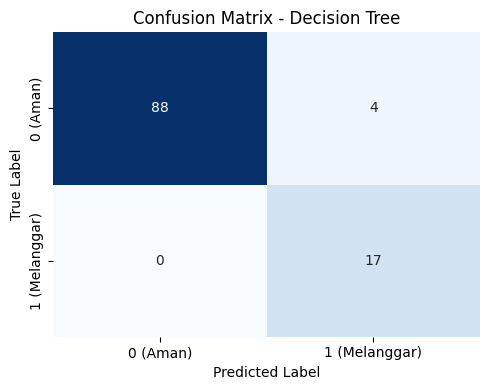
\includegraphics[width=\textwidth]{Gambar/CM_Riil_DT_Tanpa_Tuning.png}
        \caption{Tanpa Tuning}
        \label{fig:cm_dt_tanpa_tuning}
    \end{subfigure}
    \hfill
    \begin{subfigure}[b]{0.45\textwidth}
        \centering
        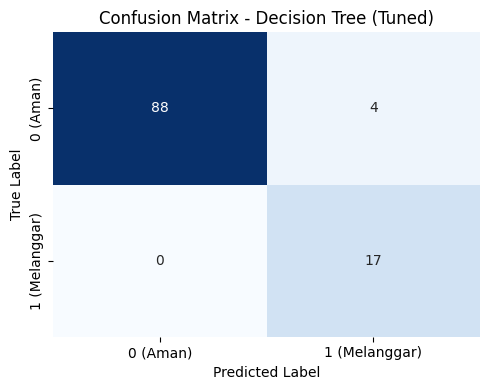
\includegraphics[width=\textwidth]{Gambar/CM_Riil_DT_Tuned.png}
        \caption{Dengan Tuning}
        \label{fig:cm_dt_tuned}
    \end{subfigure}
    \caption{Perbandingan \textit{Confusion Matrix} Model \textit{Decision Tree} (Data Riil)}
    \label{fig:cm_comparison_dt}
\end{figure}

\begin{figure}[H]
    \centering
    \begin{subfigure}[b]{0.45\textwidth}
        \centering
        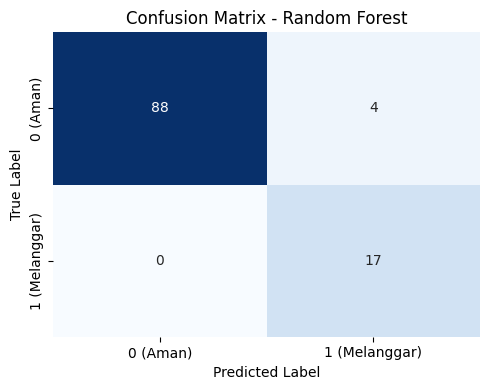
\includegraphics[width=\textwidth]{Gambar/CM_Riil_RF_Tanpa_Tuning.png}
        \caption{Tanpa Tuning}
        \label{fig:cm_rf_tanpa_tuning}
    \end{subfigure}
    \hfill
    \begin{subfigure}[b]{0.45\textwidth}
        \centering
        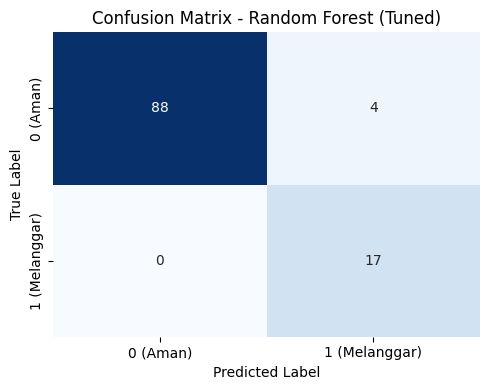
\includegraphics[width=\textwidth]{Gambar/CM_Riil_RF_Tuned.png}
        \caption{Dengan Tuning}
        \label{fig:cm_rf_tuned}
    \end{subfigure}
    \caption{Perbandingan \textit{Confusion Matrix} Model \textit{Random Forest} (Data Riil)}
    \label{fig:cm_comparison_rf}
\end{figure}

\begin{figure}[H]
    \centering
    \begin{subfigure}[b]{0.45\textwidth}
        \centering
        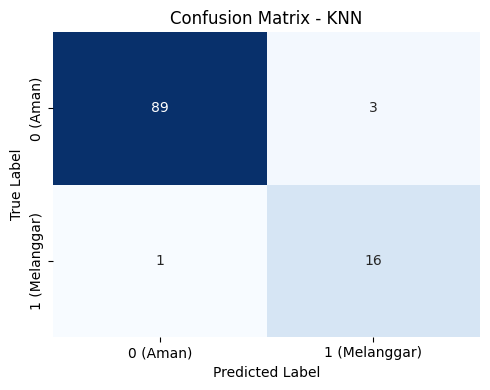
\includegraphics[width=\textwidth]{Gambar/CM_Riil_KNN_Tanpa_Tuning.png}
        \caption{Tanpa Tuning}
        \label{fig:cm_knn_tanpa_tuning}
    \end{subfigure}
    \hfill
    \begin{subfigure}[b]{0.45\textwidth}
        \centering
        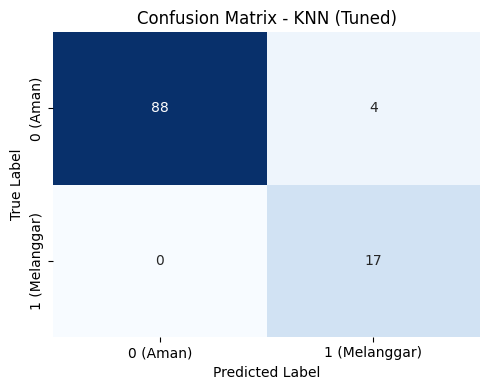
\includegraphics[width=\textwidth]{Gambar/CM_Riil_KNN_Tuned.png}
        \caption{Dengan Tuning}
        \label{fig:cm_knn_tuned}
    \end{subfigure}
    \caption{Perbandingan \textit{Confusion Matrix} Model \textit{K-Nearest Neighbors} / KNN (Data Riil)}
    \label{fig:cm_comparison_knn}
\end{figure}

\begin{figure}[H]
    \centering
    \begin{subfigure}[b]{0.45\textwidth}
        \centering
        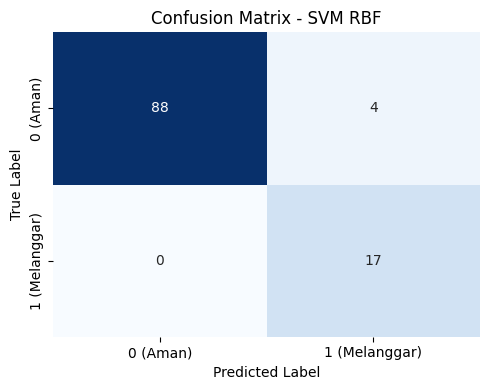
\includegraphics[width=\textwidth]{Gambar/CM_Riil_SVM_Tanpa_Tuning.png}
        \caption{Tanpa Tuning}
        \label{fig:cm_svm_tanpa_tuning}
    \end{subfigure}
    \hfill
    \begin{subfigure}[b]{0.45\textwidth}
        \centering
        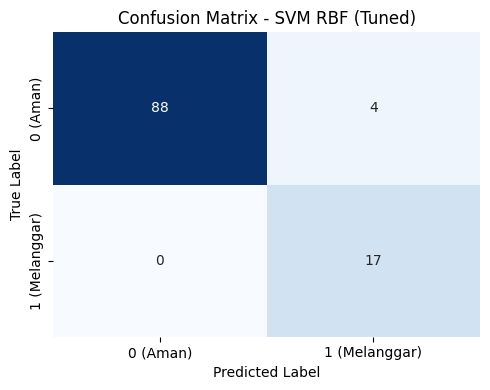
\includegraphics[width=\textwidth]{Gambar/CM_Riil_SVM_Tuned.png}
        \caption{Dengan Tuning}
        \label{fig:cm_svm_tuned}
    \end{subfigure}
    \caption{Perbandingan \textit{Confusion Matrix} Model \textit{Support Vector Machine} / SVM (Data Riil)}
    \label{fig:cm_comparison_svm}
\end{figure}

\begin{figure}[H]
    \centering
    \begin{subfigure}[b]{0.45\textwidth}
        \centering
        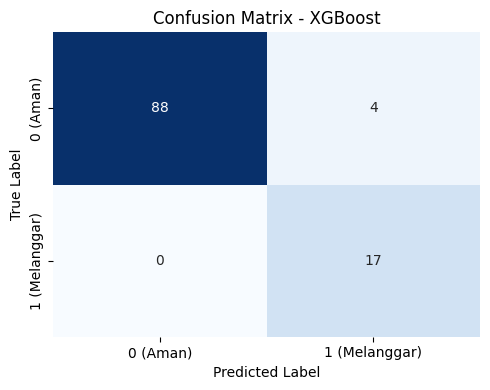
\includegraphics[width=\textwidth]{Gambar/CM_Riil_XGBoost_Tanpa_Tuning.png}
        \caption{Tanpa Tuning}
        \label{fig:cm_xgboost_tanpa_tuning}
    \end{subfigure}
    \hfill
    \begin{subfigure}[b]{0.45\textwidth}
        \centering
        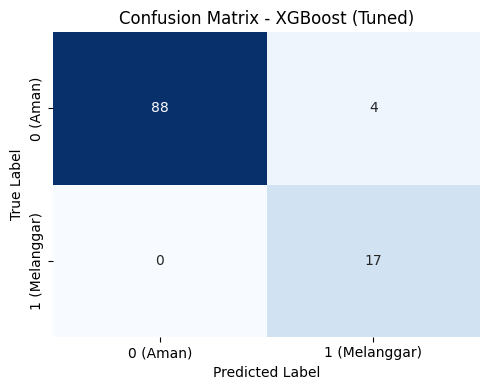
\includegraphics[width=\textwidth]{Gambar/CM_Riil_XGBoost_Tuned.png}
        \caption{Dengan Tuning}
        \label{fig:cm_xgboost_tuned}
    \end{subfigure}
    \caption{Perbandingan \textit{Confusion Matrix} Model \textit{XGBoost} (Data Riil)}
    \label{fig:cm_comparison_xgboost}
\end{figure}

Berdasarkan pemaparan di atas, maka model \textbf{\textit{XGBoost} versi tanpa tuning} ditetapkan secara resmi sebagai arsitektur klasifikasi yang akan diimplementasikan pada sistem. Keputusan ini didasarkan pada pertimbangan bahwa performa versi tanpa {\it tuning} untuk kelompok model berbasis pohon dan jarak tertentu—yakni \textit{XGBoost}, \textit{Decision Tree}, dan SVM—sudah menghasilkan performa yang sangat baik dan optimal dengan tingkat akurasi (\textbf{96,33\%}) serta \textit{Recall} kelas minoritas yang sempurna (\textbf{1,0000}). Di antara ketiga kandidat model optimal tersebut, \textit{XGBoost} dipilih karena memiliki waktu eksekusi prediksi yang paling cepat (Tabel~\ref{tab:waktu_eksekusi}). Berdasarkan hasil pengujian komputasi untuk 1000 iterasi prediksi, \textit{XGBoost} mencatatkan total waktu paling efisien sebesar 3,117823 detik dengan rata-rata waktu per prediksi 0,003118 detik. Durasi komputasi ini lebih cepat dibandingkan dengan \textit{Decision Tree} yang membutuhkan total waktu 3,254093 detik (rata-rata 0,003254 detik) dan SVM yang memerlukan total waktu 3,271034 detik (rata-rata 0,003271 detik). 

\begin{table}[H]
\centering
\caption{Perbandingan Waktu Eksekusi Prediksi Model Tanpa Tuning (1000 Iterasi)}
\label{tab:waktu_eksekusi}
\begin{tabular}{|l|c|c|}
\hline
\textbf{Model} & \textbf{Total Waktu (detik)} & \textbf{Rata-rata Waktu (detik)} \\
\hline
Decision Tree & 3,254093 & 0,003254 \\
\hline
SVM & 3,271034 & 0,003271 \\
\hline
\textbf{XGBoost} & \textbf{3,117823} & \textbf{0,003118} \\
\hline
\end{tabular}
\end{table}
Dengan demikian, konfigurasi \textit{XGBoost} tanpa tuning menjadi opsi terbaik karena mampu memberikan kecepatan pemrosesan tertinggi dalam pendeteksian anomali pelanggaran tata tertib pada sistem.

% Sub-bab 4.9 Eksport Model Terbaik
\section{Eksport Model Terbaik}

Berdasarkan hasil perbandingan evaluasi kinerja sebelumnya, model \textbf{\textit{XGBoost} versi tanpa \textit{tuning}} terbukti menghasilkan tingkat akurasi maksimal dan metrik \textit{Recall} untuk kelas minoritas yang sempurna secara efisien dengan waktu eksekusi yang paling cepat. Oleh karena itu, model \textit{XGBoost} yang diimplementasikan pada sistem. Proses ekstraksi dan penyimpanan (\textit{export}) model dilakukan menggunakan pustaka \texttt{joblib} pada bahasa pemrograman Python. Pada tahap ini, model \textit{XGBoost} digabungkan menjadi satu kesatuan bersama komponen pendukung utamanya. Komponen pendukung tersebut meliputi \textit{Label Encoder} yang berfungsi untuk melakukan transformasi dari nilai kategorikal teks menjadi format angka, serta aturan pendefinisian tiga fitur terpilih. Penggabungan komponen ini bertujuan untuk memastikan bahwa setiap data masukan (\textit{input}) baru yang dikirimkan melalui aplikasi dapat diproses dan diseragamkan formatnya secara otomatis agar sama persis dengan struktur data yang digunakan pada fase pelatihan model, sehingga mencegah terjadinya \textit{error} akibat ketidaksesuaian tipe data. Kesatuan objek tersebut kemudian disimpan ke dalam format berkas \textit{pickle} dengan nama \texttt{model\_xgboost.pkl}.

Berkas model yang telah diekstrak tersebut selanjutnya diintegrasikan secara langsung ke dalam aplikasi Data Capture. Melalui integrasi ini, aplikasi mampu memberikan klasifikasi secara langsung (\textit{real-time}) terhadap setiap data penyewa baru yang dimasukkan. Sistem akan menampilkan peringatan berupa pesan ``Penyewa Berpotensi Melakukan Pelanggaran!'' apabila seorang penyewa terklasifikasi ke dalam kelas 1, yang mengindikasikan penyewa berpotensi melakukan pelanggaran. Sebaliknya, apabila profil data penyewa yang diinput tergolong ke dalam kelas 0 (terindikasi normal dan aman), sistem tidak akan memunculkan peringatan apa pun pada layar antarmuka pengguna.
